\subsubsection{Penetration Testservice}

Das Penetration Testservice ist der Dienst, der für die Ausführung
von Penetrations- und Sicherheitstestskripten verantwortlich ist.
Dieser Dienst besteht aus einem einzigen Container:

\begin{itemize}
    \setlength\itemsep{1em}

    \item[] \textbf{Owasp}: Dieser Container besteht aus einem
    stabilen Abbild von Zapproxy und enthält die verschiedenen
    Skripte, die auf \gls{jexam_new} und \gls{jexam_2009}
    ausgeführt werden: zap-baseline und zap-fullscan.

\end{itemize}

\begin{figure}[H]
    \centering
    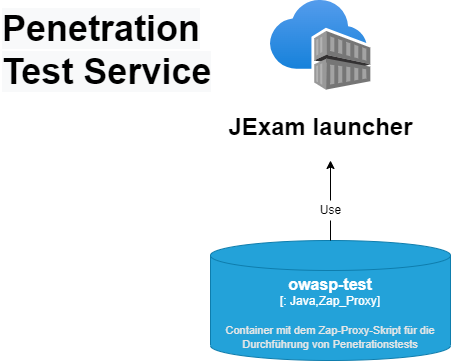
\includegraphics[scale=0.6]{images/penetration.drawio}
    \caption{jExam Penetration Testservice} \label{fig:pen}
\end{figure}